\documentclass[a4paper,11pt]{article}

\usepackage[utf8]{inputenc}

\usepackage{graphicx}
\usepackage{caption}
\usepackage{subcaption}

\usepackage{pgfplots}
\pgfplotsset{compat=1.18} 

\usepackage{minted}
\usepackage{siunitx}

\usepackage{tikz}
\usetikzlibrary{arrows.meta,calc,positioning}

\begin{document}

\title{
    \textbf{Queues in C}
}
\author{Mo Wang}
\date{Spring 2026}

\maketitle

\section*{Benchmark Results}
benchmark of raw queue - enqueue

\begin{table}[h]
\begin{center}
\begin{tabular}{l|cccccccc}
\textbf{Size}
    & 1024 & 2048 & 4196 & 8192 & 16384 & 32768 & 65536 & 131072 \\
\hline
\textbf{Time (ns)}
    & $6.8\times10^{2}$
    & $1.7\times10^{3}$
    & $4.4\times10^{3}$
    & $8.3\times10^{3}$
    & $1.5\times10^{4}$
    & $3.0\times10^{4}$
    & $6.1\times10^{4}$
    & $1.3\times10^{5}$ \\
\end{tabular}
\caption{Minimum time per loop for raw queue enqueue benchmark}
\label{tab:queue-raw-enqueue-min}
\end{center}
\end{table}

\begin{figure}[h]
  \centering
  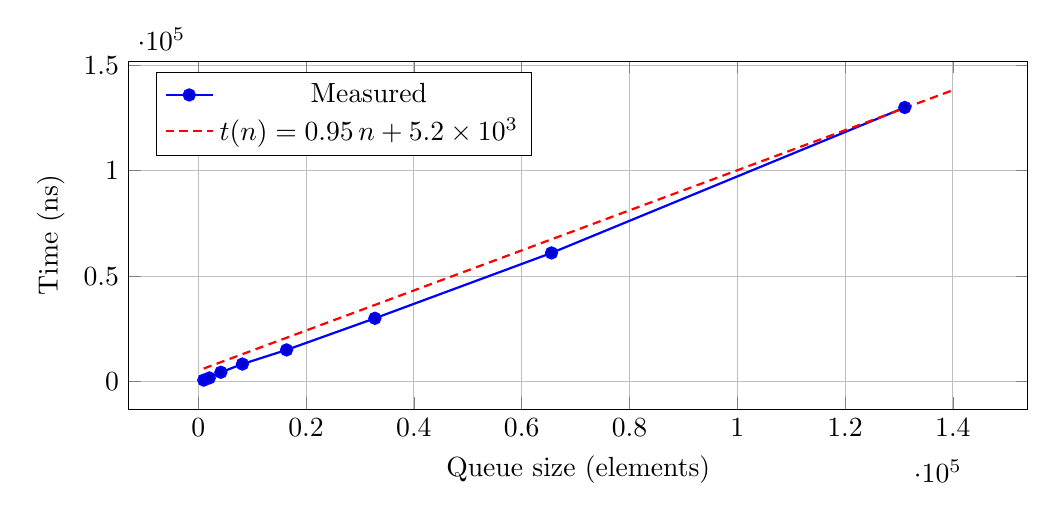
\begin{tikzpicture}
    \begin{axis}[
      xlabel={Queue size (elements)},
      ylabel={Time (ns)},
      width=13cm, height=6cm,
      grid=major,
      legend pos=north west,
      ymajorgrids=true,
      xmajorgrids=true
    ]

      % ----------------------------------------------------------
      % Measured MIN times
      % ----------------------------------------------------------
      \addplot+[
        mark=*,
        thick,
        color=blue
      ] coordinates {
        (1024,   6.8e2)
        (2048,   1.7e3)
        (4196,   4.4e3)
        (8192,   8.3e3)
        (16384,  1.5e4)
        (32768,  3.0e4)
        (65536,  6.1e4)
        (131072, 1.3e5)
      };
      \addlegendentry{Measured}

      % ----------------------------------------------------------
      % Fitted line: t(n) ≈ 0.95 n + 5.2e3
      % ----------------------------------------------------------
      \addplot[
        red,
        thick,
        densely dashed,
        domain=1000:140000,
        samples=40
      ] {0.95 * x + 5.2e3};
      \addlegendentry{$t(n)=0.95\,n + 5.2\times10^{3}$}

    \end{axis}
  \end{tikzpicture}
  \caption{Raw queue enqueue: minimum time per loop with fitted linear regression}
  \label{fig:queue-raw-enqueue-min-fitted}
\end{figure}


benchmark of raw queue - dequeue
\begin{table}[h]
\begin{center}
\begin{tabular}{l|cccccccc}
\textbf{Size}
    & 1024 & 2048 & 4196 & 8192 & 16384 & 32768 & 65536 & 131072 \\
\hline
\textbf{Time (ns)}
    & 8.1 & 8.3 & 8.4 & 8.3 & 8.2 & 8.0 & 8.2 & 8.1 \\
\end{tabular}
\caption{Raw queue \texttt{dequeue}: minimum time per loop}
\label{tab:queue-dequeue-min}
\end{center}
\end{table}

\begin{figure}[h]
  \centering
  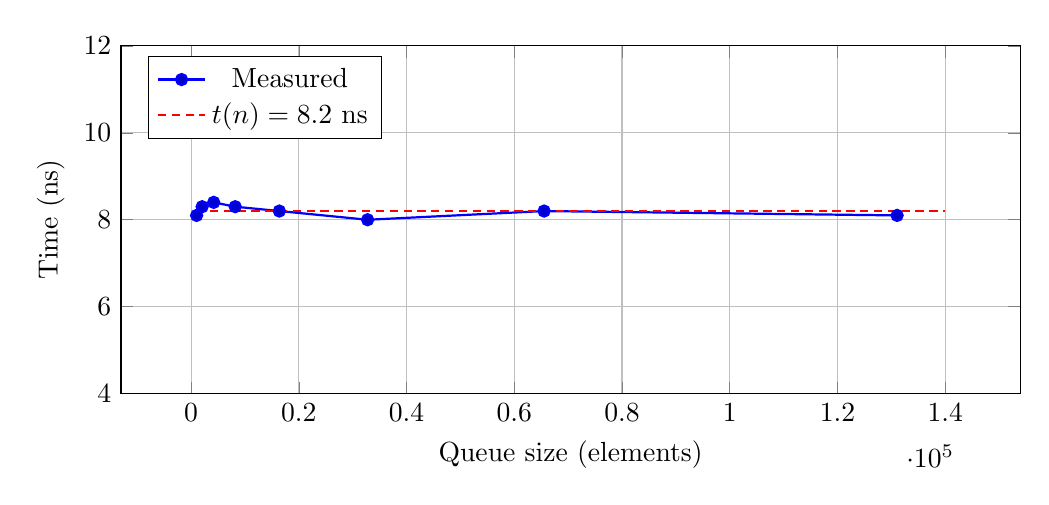
\begin{tikzpicture}
    \begin{axis}[
      xlabel={Queue size (elements)},
      ylabel={Time (ns)},
      width=13cm, height=6cm,
      grid=major,
      legend pos=north west,
      ymajorgrids=true,
      xmajorgrids=true,
      ymin=4, ymax=12
    ]

      % ---------------------------
      % Measured MIN times
      % ---------------------------
      \addplot+[
        mark=*,
        thick,
        color=blue
      ] coordinates {
        (1024,    8.1)
        (2048,    8.3)
        (4196,    8.4)
        (8192,    8.3)
        (16384,   8.2)
        (32768,   8.0)
        (65536,   8.2)
        (131072,  8.1)
      };
      \addlegendentry{Measured}

      % ---------------------------
      % Constant fit: t(n) ≈ 8.2 ns
      % ---------------------------
      \addplot[
        red,
        thick,
        densely dashed,
        domain=900:140000,
        samples=2
      ] {8.2};
      \addlegendentry{$t(n)=8.2\ \text{ns}$}

    \end{axis}
  \end{tikzpicture}
  \caption{Raw queue \texttt{dequeue}: minimum time per loop with constant fit}
  \label{fig:queue-dequeue-min-fit}
\end{figure}

benchmark of improved queue - enqueue
\begin{table}[h]
\begin{center}
\begin{tabular}{l|ccccccccc}
\textbf{Size}
    & 1024 & 2048 & 4196 & 8192 & 16384 & 32768 & 65536 & 131072 & 262144 \\
\hline
\textbf{Time (ns)}
    & 7.8
    & 7.9
    & 7.9
    & 8.0
    & 8.1
    & 8.0
    & 8.1
    & 8.0
    & 8.2 \\
\end{tabular}
\caption{Improved queue \texttt{enqueue}: minimum time per loop}
\label{tab:improved-queue-enqueue-min}
\end{center}
\end{table}

\begin{figure}[h]
  \centering
  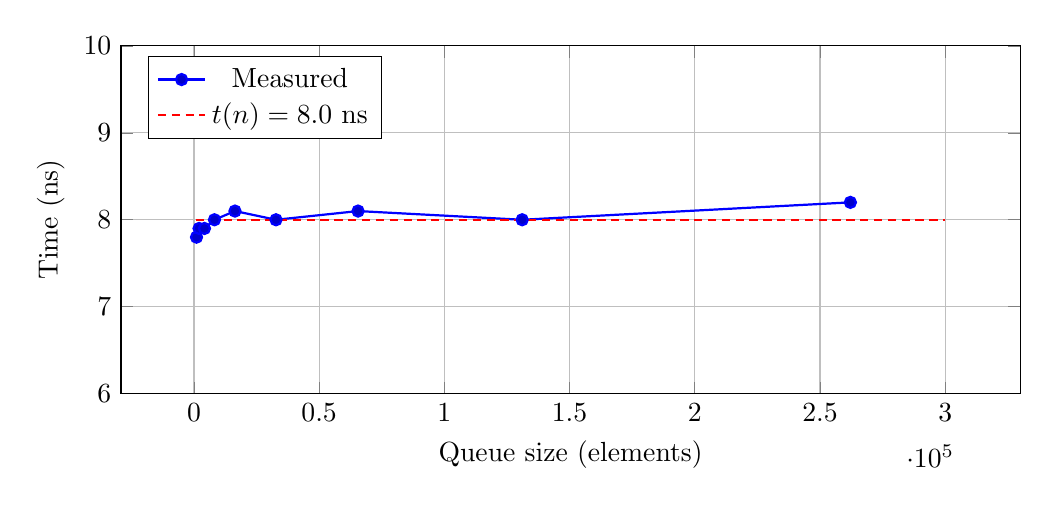
\begin{tikzpicture}
    \begin{axis}[
      xlabel={Queue size (elements)},
      ylabel={Time (ns)},
      width=13cm, height=6cm,
      grid=major,
      legend pos=north west,
      ymajorgrids=true,
      xmajorgrids=true,
      ymin=6, ymax=10   % optional: enlarge Y range as you requested
    ]

      % ----------------------------------------------------------
      % Measured MIN times
      % ----------------------------------------------------------
      \addplot+[
        mark=*,
        thick,
        color=blue
      ] coordinates {
        (1024,    7.8)
        (2048,    7.9)
        (4196,    7.9)
        (8192,    8.0)
        (16384,   8.1)
        (32768,   8.0)
        (65536,   8.1)
        (131072,  8.0)
        (262144,  8.2)
      };
      \addlegendentry{Measured}

      % ----------------------------------------------------------
      % Constant fit: t(n) = 8.0 ns
      % ----------------------------------------------------------
      \addplot[
        red,
        thick,
        densely dashed,
        domain=800:300000,
        samples=2
      ] {8.0};
      \addlegendentry{$t(n)=8.0\ \text{ns}$}

    \end{axis}
  \end{tikzpicture}
  \caption{Improved queue \texttt{enqueue}: minimum time per loop with constant fit}
  \label{fig:improved-queue-enqueue-min-fit}
\end{figure}


benchmark of improved queue - dequeue
\begin{table}[h]
\begin{center}
\begin{tabular}{l|cccccccc}
\textbf{Size}
    & 1024 & 2048 & 4196 & 8192 & 16384 & 32768 & 65536 & 131072 \\
\hline
\textbf{Time (ns)}
    & 8.4  & 8.4  & 8.5  & 8.4  & 8.5   & 8.3   & 8.9   & 8.4 \\
\end{tabular}
\caption{Improved queue \texttt{dequeue}: minimum time per loop}
\label{tab:improved-queue-dequeue-min}
\end{center}
\end{table}

\begin{figure}[h]
  \centering
  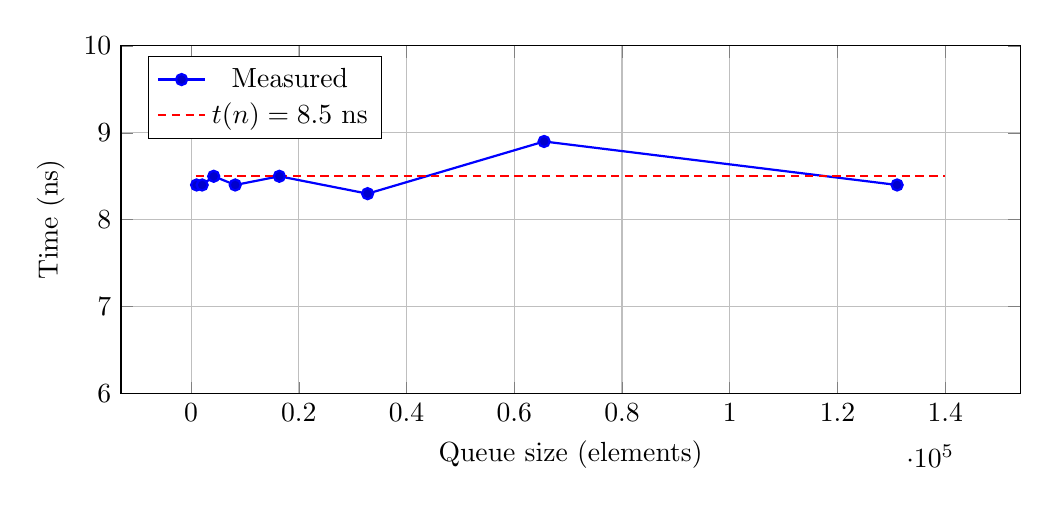
\begin{tikzpicture}
    \begin{axis}[
      xlabel={Queue size (elements)},
      ylabel={Time (ns)},
      width=13cm, height=6cm,
      grid=major,
      legend pos=north west,
      ymajorgrids=true,
      xmajorgrids=true,
      ymin=6, ymax=10,
      ytick={6,7,8,9,10}
    ]

      % ---------------------------
      % Measured MIN times
      % ---------------------------
      \addplot+[
        mark=*,
        thick,
        color=blue
      ] coordinates {
        (1024,    8.4)
        (2048,    8.4)
        (4196,    8.5)
        (8192,    8.4)
        (16384,   8.5)
        (32768,   8.3)
        (65536,   8.9)
        (131072,  8.4)
      };
      \addlegendentry{Measured}

      % ---------------------------
      % Constant fit: t(n) = 8.5 ns
      % ---------------------------
      \addplot[
        red,
        thick,
        densely dashed,
        domain=900:140000,
        samples=2
      ] {8.5};
      \addlegendentry{$t(n)=8.5\ \text{ns}$}

    \end{axis}
  \end{tikzpicture}
  \caption{Improved queue \texttt{dequeue}: minimum time per loop with constant fit}
  \label{fig:improved-queue-dequeue-min-fit}
\end{figure}


Wrap Queue:
\begin{figure}[h]
\centering
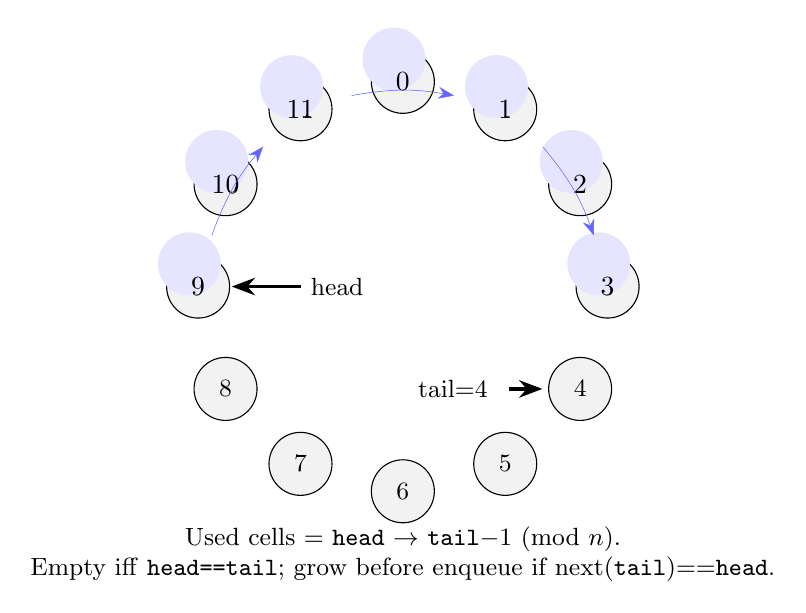
\begin{tikzpicture}[
  >=Stealth,
  slot/.style={draw, circle, minimum size=8mm, inner sep=0pt, font=\small},
  used/.style={fill=blue!10},
  free/.style={fill=gray!10},
  pointer/.style={->, very thick},
  label/.style={font=\small}
]

% --- parameters ---
\def\n{12}         % capacity
\def\R{2.6}        % ring radius
\def\head{9}       % head index
\def\tail{4}       % first free slot
% Example: used indices = 9,10,11,0,1,2,3 (head..tail-1 mod n)

% --- place slots on a circle ---
\foreach \i in {0,...,11} {
  \coordinate (c\i) at ({90 - (360/\n)*\i}:\R);
  \node[slot,free] (s\i) at (c\i) {\i};
}

% --- color used range ---
\foreach \i in {9,10,11,0,1,2,3} {
  \begin{scope}
    \fill[blue!10] (s\i.north east) arc[start angle=0,end angle=360,radius=4mm] -- cycle;
    % overlay the index again for clarity
    \node at (s\i) {\i};
  \end{scope}
}

% --- head & tail arrows ---
% --- HEAD label to the right of circle 9, arrow into circle 9 ---
% Text label placed 9 mm to the right of the circle's east anchor:
\node[font=\small, anchor=west] (headlabel) at ($(s9.east)+(9mm,0)$) {head};
% Arrow from the label back into the circle's right side:
\draw[->, very thick]
  (headlabel.west) -- ($(s9.east)+(0.2mm,0)$);

\draw[pointer] ($(s\tail)+(-0.9,0)$) -- ($(s\tail)+(-0.48,0)$);
\node[label,left] at ($(s\tail)+(-1.05,0)$) {tail=\tail};

% --- arc annotation for the used segment ---
\draw[very thin, blue!60, -{Stealth[length=2mm]}]
  ($(s\head)!0.5!(s10)$) to[bend left=10] ($(s10)!0.5!(s11)$);
\draw[very thin, blue!60, -{Stealth[length=2mm]}]
  ($(s11)!0.5!(s0)$) to[bend left=10] ($(s0)!0.5!(s1)$);
\draw[very thin, blue!60, -{Stealth[length=2mm]}]
  ($(s1)!0.5!(s2)$) to[bend left=10] ($(s2)!0.5!(s3)$);

\node[align=center, font=\small, fill=white, inner sep=1pt] at (0,-3.4) {%
Used cells = \texttt{head} $\rightarrow$ \texttt{tail}$-1$ (mod $n$).\\
Empty iff \texttt{head==tail}; grow before enqueue if next(\texttt{tail})==\texttt{head}.
};

\end{tikzpicture}
\caption{Wrap-around queue shown as a ring: indices advance modulo $n$; the used segment runs from head to tail$-1$.}
\label{fig:wrap-queue-ring}
\end{figure}


\end{document}